\documentclass[12pt,a4paper]{article}
\usepackage[utf8x]{inputenc}
\usepackage{ucs}
\usepackage{amsmath}
\usepackage{amsfonts}
\usepackage{amssymb}
\usepackage{graphicx}
\usepackage{grffile}
\usepackage{float}
\usepackage[portuguese]{babel}
\title{Trabalho 6}
\author{André Garnier Coutinho}
\setlength{\textwidth}{17cm}
\setlength{\textheight}{24cm}
\addtolength{\topmargin}{-2cm}
\addtolength{\oddsidemargin}{-2cm}
\begin{document}
\begin{center}
\textbf{Instituto de Matemática e Estatística da USP\linebreak MAT 2455 - Cálculo Diferencial e Integral III para Engenharia\linebreak Trabalho 6 - 1º semestre de 2012}
\end{center}



\noindent{\bf Questão 1.} (2 pontos) Calcule

\[ \iint_{s} ( \ln (1+z^8) + 2x \sin(2y)) dy \wedge dz + (\cos(2y))dz \wedge dx + (z^2 - yx^2)dx \wedge dy \]
onde $S$ é parte da superfície $z = 4 - 2x^2 - y^2 $ limitada pelo plano $z = 0$, orientada com $ \vec{N} \cdot \vec{k} \geq 0 $. (atenção: a superfície $S$ não é fechada).

\noindent{\bf \\Solução:}

Seja $S_1$ parte do plano $z=0$ que fecha a superfície $S$. Seja $V$ definida pelo interior de $S \cup S_1 $ e orientada com vertor normal  para fora de $V$, ou seja, para fora da superfície fechada $S \cup S_1$

Como o domínio de $\vec{F} $ não apresenta singularidades na região $V$, pelo Teorema de Gauss:

\[ \iint_{S} \vec{F}  \cdot \vec{N} \,dS + \iint_{ S_1 } \vec{F}  \cdot \vec{N} \,dS = \iiint_{V} div(\vec{F})  \,dx \,dy \,dz  \]



\begin{equation}
\iint_{S} \vec{F}  \cdot \vec{N} \,dS = - \iint_{ S_1 } \vec{F}   \cdot \vec{N} \,dS  + \iiint_{V} div(\vec{F}) \,dx \,dy \,dz
\label{eq:1}
\end{equation} \\


\begin{figure}[h!]
	\centering
	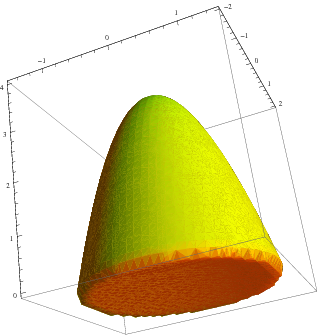
\includegraphics[scale=0.5]{1a.png}  
	\caption{Região V e superfícies $S$ e $S_1$ }
	\label{fig:figura1}
\end{figure} \\

A superfície $S_1$ pode ser facilmente parametrizada da seguinte forma:

\[ \sigma (u,v) = (u, v, 0) \] 

Para encontrar os valores de $(u,v)$ em que a superfície $S_1$ é definida, encontramos a intersecção do plano com o parabolóide. Assim temos:

\[ \left\{\begin{array}{ll}
z = 0 \\
z = 4- 2x^2 + y^2
\end{array}\right. \Rightarrow \left\ {\begin{array}{ll}

2x^2 + y^2 = 4   \end{array} \right. \]





Sendo assim, temos que a região $R$ na qual a superfície $S_1$ é definida é: \\
\[ R = \{ (u,v) \in \mathbb{R}^2 \hspace{1 mm} | \hspace{1 mm}  2u^2 + v^2 \leq 4 \} \]

Calculando o vetor $\sigma_x \wedge \sigma_y$:

\[ \sigma_u = (1,0, 0 ) \]
\[ \sigma_v = (0,1, 0 ) \]
\[  \sigma_u \wedge \sigma_v = ( 0, 0, 1 ) \] 

Como a normal da superfície $S_1$ é aponta para baixo e $\sigma_u \wedge \sigma_v$ aponta para cima, invertemos o sinal de $\sigma_u \wedge \sigma_v$ para calcular a integral de superfície. Assim:



\[ \iint_{S_1} \vec{F}  \cdot \vec{N} \,dS = \iint_{R} (0 + 2u \sin(2v), \cos(2v), 0 - vu^2) \cdot (0, 0, -1) \,du \,dv = \iint_{R}   vu^2 \,du \,dv  \]

Como a região $R$ é simetríca em $v$ e o integrando é uma função ímpar em $v$


\begin{equation}
\iint_{R} \vec{F}  \cdot \vec{N} \,dS = 0
\label{eq:2}
\end{equation} \\

\[ div(\vec{F}) =  \frac{\partial P}{\partial x} + \frac{\partial Q}{\partial y} + \frac{\partial R}{\partial z}  = 2\sin(2y) - 2\sin(2y) + 2z =  2z \]

\[ \iiint_{V} div(\vec{F}) \,dx \,dy \,dz = \iint_{R} \Big( \int_{0}^{4 - 2x^2 - y^2} 2z \,dz \Big) \,dx \,dy = \iint_{R} \Big(  z^2 \Big|_{0}^{4 - 2x^2 - y^2}  \Big) \,dx \,dy  \]

\[ = \iint_{R} (4 - 2x^2 - y^2 )^2 \,dx \,dy \]

Realizando a seguinte mudança de coordenadas:
\begin{equation}
\left\{\begin{array}{ll}
x= \sqrt{2} \rho\cos\theta\\
y=2\rho\sin\theta
\end{array}\right.
\label{eq:mudanca}
\end{equation}

\[ |J| = 2 \sqrt{2} \rho \]

\[ = \int_{0}^{2 \pi} \int_{0}^{1} 2 \sqrt{2} \rho (4 - 4 \rho^2 \cos^2 \theta - 4 \rho^2 \sin^2 \theta )^2 \,d\rho \,d\theta =  2 \sqrt{2} \int_{0}^{2 \pi} \int_{0}^{1}  \rho (4 - 4 \rho^2)^2 \,d\rho \,d\theta \]

\[ 2 \sqrt{2} \cdot 2\pi \cdot 16 \int_{0}^{1}  \rho (1 -2\rho^2 + 1 \rho^4) \,d\rho = 64 \sqrt{2} \pi \Big( \frac{\rho^2}{2} - 2 \frac{\rho^4}{4} + \frac{\rho^6}{6} \Big)_{0}^{1} \]

\begin{equation}
\therefore \iiint_{R} div(\vec{F}) \,dx \,dy \,dz = \frac{32 \sqrt{2} \pi}{3}
\label{eq:3}
\end{equation} \\

Substituindo (\ref{eq:2}) e (\ref{eq:3}) em (\ref{eq:1}):

\[ \iint_{S} \vec{F}  \vec{N} \,dS = - 0 + \frac{32 \sqrt{2} \pi}{3} = \frac{32 \sqrt{2} \pi}{3}  \]
 




\newpage

\noindent{\bf Questão 2.} (3,5 pontos) Calcule $\displaystyle \int_{\gamma} \vec{F}  \cdot d\vec{r} $ sendo $ \displaystyle \vec{F} = \Big( e^{z^2} + \frac{-y}{x^2 + y^2}, x^2 + \frac{x}{x^2 + y^2}, 2xze^{z^2} \Big)}$  e $\gamma $  a intersecção de $z = x^2 + y^2$ e $z = 4 -x^2$, orientada de modo que a projeção no plano $0xy$ é percorrida no sentido anti-horário.

\noindent{\bf \\Solução:}

Podemos decompor $\vec{F}$ na soma de dois campos vetoriais $\vec{F_1}$ e $\vec{F_2}$, sendo:

\[ \vec{F_1} =  \Big( \frac{-y}{x^2 + y^2}, \frac{x}{x^2 + y^2}, 0 \Big) ; \vec{F_2} = ( e^{z^2}, x^2, 2xze^{z^2} ) \] \\

Calculando os rotacionais de $\vec{F_1}$ e $\vec{F_2}$:

\[ \displaystyle Rot(\vec{F_1}) =  \begin{vmatrix} \vec{i} & \vec{j} & \vec{k} \\ \frac{\partial}{\partial x} & \frac{\partial}{\partial y} & \frac{\partial}{\partial z}  \\ \frac{-y}{x^2 + y^2}  & \frac{x}{x^2 + y^2} & 0  \end{vmatrix} = \Big( \frac{1 \cdot (4x^2 + y^2) - x \cdot (8x)}{(4x^2 + y^2)^2} - \frac{(-1) \cdot (4x^2 + y^2) - (-y) \cdot (2y)}{(4x^2 + y^2)^2} \Big) \^{k} = \vec{0} \] 

\[ Rot(\vec{F_2}) = \begin{vmatrix} \vec{i} & \vec{j} & \vec{k} \\ \frac{\partial}{\partial x} & \frac{\partial}{\partial y} & \frac{\partial}{\partial z}  \\  e^{z^2} & x^2 & 2xze^{z^2}  \end{vmatrix} = 0\vec{i} + (2ze^{z^2} - 2ze^{z^2})\vec{j} + 2x\vec{k} = 2x\vec{k} \]  \\

Como $\gamma$ é uma curva fechada e, o domínio de $\vec{F_2}$ é simplesmente conexo, podemos utilizar o teorema de Stokes para calcular $ \displaystyle \int_{\gamma} \vec{F_2} \cdot d\vec{r} $, escolhendo como superfície  $z = 4 - x^2$ limitada por $z = x^2 + y^2 $, a qual chamaremos de $S_2$ . \\

Como a projeção de $\gamma $ em $0xy$ é no sentido-horário, temos que a normal induzida pelo Teorema de Stokes em $S_2$ tem a componente na direção $\vec{k}$ positiva. Assim, parametrizando $S_2$: 

\[ \sigma (u,v) = (u,v, 4-u^2) \] \\
Para encontrar os valores de $(u,v)$ em que a superfície $S_2$ é definida, encontramos a intersecção da calha com o parabolóide. Assim temos:

\[ \left\{\begin{array}{ll}
z = 4 - x^2 \\
z = x^2 + y^2
\end{array}\right. \Rightarrow \left\ {\begin{array}{ll}

2x^2 + y^2 = 4   \end{array} \right. \]


Sendo assim, temos que a região $R_2$ na qual a superfície $S_2$ é definida é: \\
\[ R_2 = \{ (u,v) \in \mathbb{R}^2 \hspace{1 mm} | \hspace{1 mm}  2u^2 + v^2 \leq 4 \} \]

Calculando o vetor $\sigma_{u} \wedge \sigma_{v}$:

\[ \sigma_u = (1,0, -2u ) \]
\[ \sigma_v = (0,1, 0 ) \]
\[  \sigma_u \wedge \sigma_v = ( 2u, 0, 1 ) \] 

Como $\sigma_u \wedge \sigma_v$ está no mesmo sentido da normal de $S_2$, aplicando o Teorema de Stokes, temos:

\[ \int_{\gamma} \vec{F_2} \cdot d\vec{r} = \iint_{S_2} Rot(\vec{F_2}) \cdot \vec{N} \,dS = \iint_{R_2} (0, 0, 2u) \cdot ( 2u, 0, 1 )  \,du \,dv =  \iint_{R_2} 2u \,du \,dv\]

Como a região $R_2$ é simetríca em $u$ e o integrando é uma função ímpar em $u$:

\[ \iint_{R_2} 2u \,du \,dv\ = 0 \Rightarrow  \int_{\gamma} \vec{F_2} \cdot d\vec{r} = 0 \] \\

Assim, como $ \displaystyle  \int_{\gamma} \vec{F} \cdot d\vec{r} =  \int_{\gamma} \vec{F_1} \cdot d\vec{r} +  \int_{\gamma} \vec{F_2} \cdot d\vec{r} $, temos que $ \displaystyle \int_{\gamma} \vec{F} \cdot d\vec{r} =  \int_{\gamma} \vec{F_1} \cdot d\vec{r} $. \\

Para calcular $ \displaystyle \int_{\gamma} \vec{F_1} \cdot d\vec{r} $, não podemos escolher uma superfície que seja cortada pelo eixo $z$ quando aplicarmos o Teorema de Stokes, pois $\vec{F_1}$ não é definido para pontos do tipo $(0,0,z), z \in \mathbb{R} $. \\

Sendo assim, escolhemos a superfície cilindrica $2x^2 + y^2 = 4$ limitada por $z = 0 $ e $z = 4 - x^2 $, a qual chamaremos de $S_1$ sendo $\gamma$ e $\gamma_1$ os bordos do cilindro. Como a projeção de $\gamma $ em $0xy$ é no sentido horário, temos que a normal induzida pelo Teorema de Stokes em $S_1$ aponta para dentro do cilindro, o que induz uma orientação no sentido horário para $ \gamma_1$ . Assim, aplicando o Teorema de Stokes:

\[  \int_{\gamma} \vec{F_1} \cdot d\vec{r} + \int_{\gamma_1} \vec{F_1} \cdot d\vec{r} = \iint_{S_1} Rot(\vec{F_1}) \cdot \vec{N} \,dS = 0 \]


\[ \therefore \int_{\gamma} \vec{F_1} \cdot d\vec{r} = - \int_{\gamma_1} \vec{F_1} \cdot d\vec{r} \]

A região interna a $\gamma_1$ contém o ponto $(0,0,0)$, o qual é uma singularidade de $\vec{F_1}$. Então vamos usar o Teorema de Green (pois a região é plana) para calcular a integral.
Seja a curva $\gamma_2 (t) = ( \cos t, \sin t, 0), t \in [0, 2 \pi] $ a qual isola a singularidade e não se cruza com  $\gamma_1$.
Seja $D$ a região do plano $z=0$ limitada pelas curvas $\gamma_1$ e $\gamma_2$.

Para aplicar o Teorema invertemos os sinais das integrais de linha. Assim, aplicando o Teorema de Stokes (ou Green):

\[ - \int_{\gamma_1} \vec{F_1} \cdot d\vec{r} - \int_{\gamma_2} \vec{F_1} \cdot d\vec{r} = \iint_{D} Rot(\vec{F_1}) \cdot \^{k} \,dx \,dy = 0 \]

\[ \therefore \int_{\gamma_1} \vec{F_1} \cdot d\vec{r} = - \int_{\gamma_2} \vec{F_1} \cdot d\vec{r} = - \int_{0}^{2 \pi} \Big( \frac{-\sin t}{\cos^2 t + \sin^2 t} , \frac{\cos t }{\cos^2 t + \sin^2 t} , 0 \Big) \cdot (-\sin t , \cos t, 0 ) \,dt \]

\[ = - \int_{0}^{2 \pi} \Big( \sin^2 t +  \cos^2 t \Big) \,dt = - 2\pi \]

\[ \therefore \int_{\gamma} \vec{F} \cdot d\vec{r} = 2\pi \]

\newpage

\noindent{\bf Questão 3.} (2 pontos) Sejam $\displaystyle \vec{F} = \Big(\frac{-y}{x^2 + y^2},  \frac{x}{x^2 + y^2}, \cos(z^4) \Big)}$ e $\gamma $  a intersecção de $z = x^2 + \frac{y^2}{4}$ e $z + y + 2x = 1 $, orientada de modo que a projeção no plano $0xy$ é percorrida no sentido anti-horário. Um aluno utilizou o Teorema de Stokes para calcular a integral $ \displaystyle \int_{\gamma} \vec{F} \cdot d\vec{r}$. \\ Obteve $Rot(\vec{F}) = 0$ e usando $S$ a parte do plano limitado por $z = x^2 + \frac{y^2}{4}$ concluiu que

\[ \int_{\gamma} \vec{F} \cdot d\vec{r} = \iint_{S} Rot(\vec{F}) \cdot \vec{N} \,dS = 0. \]

No entanto o aluno errou o exercício.

\begin{itemize}
	\item[(a)] Comente o(s) erro(s) cometidos pelo aluno e resolva o exercício corretamente.
	
	\item[(b)] O campo é conservativo? Justifique sua resposta.
	
	
	

\end{itemize}


\noindent{\bf \\Solução:}

\begin{itemize}
	\item[(a)]Para calcular $ \displaystyle \int_{\gamma} \vec{F} \cdot d\vec{r} $, não podemos escolher uma superfície que seja cortada pelo eixo $z$ quando aplicamos o Teorema de Stokes, pois $\vec{F}$ não é definido para pontos do tipo $(0,0,z), z \in \mathbb{R} $. O erro do aluno consiste em escolher uma superfície que é cortada pelo eixo $z$. \\
	
	% O erro cometido pelo aluno foi que para aplicar o teorema de Stokes a superfície $S$ não pode conter pontos onde o campo $\vec{F}$ não é definido. Como $\vec{F}$ não é definido para pontos do tipo $(0,0,z), z \in \mathbb{R}$, $\vec{F}$ não é definido para nenhum ponto do eixo $z$. A superfície escolhida pelo aluno é cortada pelo eixo $z$, logo não poderia ter sido escolhida para aplicar o Teorema de Stokes. \\ %
	
Aqui segue a resolução correta do problema em questão: \\



Podemos decompor $\vec{F}$ na soma de dois campos vetoriais $\vec{F_1}$ e $\vec{F_2}$, sendo:

\[ \vec{F_1} =  \Big( \frac{-y}{x^2 + y^2}, \frac{x}{x^2 + y^2}, 0 \Big) ; \vec{F_2} = ( 0, 0, \cos(z^4) ) \] \\

Calculando os rotacionais de $\vec{F_1}$ e $\vec{F_2}$:

\[ \displaystyle Rot(\vec{F_1}) =  \begin{vmatrix} \vec{i} & \vec{j} & \vec{k} \\ \frac{\partial}{\partial x} & \frac{\partial}{\partial y} & \frac{\partial}{\partial z}  \\ \frac{-y}{x^2 + y^2}  & \frac{x}{x^2 + y^2} & 0  \end{vmatrix} = \Big( \frac{1 \cdot (4x^2 + y^2) - x \cdot (8x)}{(4x^2 + y^2)^2} - \frac{(-1) \cdot (4x^2 + y^2) - (-y) \cdot (2y)}{(4x^2 + y^2)^2} \Big) \^{k} = \vec{0} \] 

\[ Rot(\vec{F_2}) = \begin{vmatrix} \vec{i} & \vec{j} & \vec{k} \\ \frac{\partial}{\partial x} & \frac{\partial}{\partial y} & \frac{\partial}{\partial z}  \\  0 & 0 & \cos(z^4)  \end{vmatrix} = \vec{0} \] \\

Como $\gamma$ é uma curva fechada e, o domínio de $\vec{F_2}$ é simplesmente conexo e, $Rot(\vec{F_2}) = \vec{0}$, temos que $ \displaystyle \int_{\gamma} \vec{F_2} \cdot d\vec{r} = 0 $. \\

Como o rotacional de $\vec{F_1}$ é nulo, não precisaremos nos preocupar com a integral de superfície que aparecerá no teorema de Stokes. Sendo assim, precisamos apenas escolher uma superfície $S$ que não seja cortada pelo eixo $z$ para podermos aplicar o teorema. Uma superfície conviente seria uma superfície cilindrica limitada inferiormente por $z=0$ e superiormente por $\gamma$, a qual podemos achar fazendo a intersecção de $z = x^2 + \frac{y^2}{4}$ e $z = 1 - 2x - y$:

\[ \left\{\begin{array}{ll}
z = x^2 + \frac{y^2}{4} \\
z = 1 - 2x - y
\end{array}\right. \Rightarrow \left\ {\begin{array}{ll}

x^2 + \frac{y^2}{4} = 1 - 2x - y \Rightarrow x^2 + 2x + \frac{y^2}{4} + y = 1  \end{array} \right. \]

\[ (x +1)^2 + \Big(y + \frac{1}{2}\Big)^2 = \frac{9}{4} \]


Seja $\gamma_1$ o outro bordo do cilindro. Como a projeção de $\gamma $ em $0xy$ é no sentido-horário, temos que a normal induzida pelo Teorema de Stokes em $S$ aponta para dentro do cilindro, o que induz uma orientação no sentido horário para $ \gamma_1$ . Assim, aplicando o Teorema de Stokes:

\[  \int_{\gamma} \vec{F_1} \cdot d\vec{r} + \int_{\gamma_1} \vec{F_1} \cdot d\vec{r} = \iint_{S} Rot(\vec{F_1}) \cdot \vec{N} \,dS = 0 \]


\[ \therefore \int_{\gamma} \vec{F_1} \cdot d\vec{r} = - \int_{\gamma_1} \vec{F_1} \cdot d\vec{r} \]

A região interna a $\gamma_1$ contém o ponto $(0,0,0)$, o qual é uma singularidade de $\vec{F}$. Então adicionamos a curva $\gamma_2 (t) = a( \cos t, \sin t, 0), t \in [0, 2 \pi] $, com $a$ suficientemente pequeno de modo que $\gamma_2$ não se cruze com  $\gamma_1$, isolando assim a singularidade.


Como $\gamma_1$ e $\gamma_2$ estão no sentido contrário ao da hipótese do Teorema de Green (ou Stokes, pois a região é plana), para aplicar o teorema invertemos os sinais das integrais de linha. Assim, aplicando o Teorema de Green:

\[ - \int_{\gamma_1} \vec{F_1} \cdot d\vec{r} - \int_{\gamma_2} \vec{F_1} \cdot d\vec{r} = \iint_{R} Rot(\vec{F_1}) \cdot \^{k} \,dx \,dy = 0 \]

\[ \therefore \int_{\gamma_1} \vec{F_1} \cdot d\vec{r} = - \int_{\gamma_2} \vec{F_1} \cdot d\vec{r} = - \int_{0}^{2 \pi} \Big( \frac{-a\sin t}{a^2\cos^2 t + a^2\sin^2 t} , \frac{a\cos t }{a^2\cos^2 t + a^2\sin^2 t} , 0 \Big) \cdot (-a\sin t , a\cos t, 0 ) \,dt \]

\[ = - \int_{0}^{2 \pi} \Big( \sin^2 t +  \cos^2 t \Big) \,dt = - 2\pi \]

\[ \therefore \int_{\gamma} \vec{F} \cdot d\vec{r} = 2\pi \]

	\item[(b)] O campo não é conservativo, pois no item $(a)$ calculamos a integral de linha de $\vec{F}$ em uma curva fechada e o resultado foi diferente de zero.

 \end{itemize}


\end{document}
